\section{Related Work}

\subsection{Video-to-Motion Generation}

The field of human motion generation has progressed from action-label conditioning and music-conditioned synthesis toward video-conditioned approaches. Action-conditioned methods generate motions from categorical labels or seed poses, operating entirely within the training distribution. Degardin et al. propose a generative adversarial graph convolutional network that synthesizes human actions conditioned on discrete class labels, yet the model cannot extrapolate beyond the 10--15 action categories present during training~\cite{gagcn2021}. Similarly, Action2Motion~\cite{act2mo2020} employs a VAE-transformer architecture to generate 3D motions from action categories, but the generated repertoire remains bounded by the predefined set of 30 actions in the NTU RGB+D dataset. These approaches share a fundamental limitation: the conditioning signal is a one-hot or learned embedding of a seen category. The model learns a mapping from label to motion distribution but acquires no mechanism to compose unseen behaviors. The vocabulary of actions is closed at training time.

Data-driven generative approaches---such as text-to-motion diffusion models~\cite{motiondiffuse2022} and music-conditioned dance generation~\cite{edge2023}---offer scalable alternatives but inherit biases from limited datasets like AMASS~\cite{amass2019}, Human3.6M~\cite{h3wb2014}, and AIST++~\cite{aist2021}. Models trained on narrow domains struggle to generalize to styles such as classical dance or martial arts, reflecting the ongoing scarcity and high cost of collecting diverse 3D motion data.

\paragraph{Pose estimation from videos.}
Reconstructing 3D pose from monocular video follows a two-stage pipeline: detect 2D keypoints, then lift to 3D via convolutional or graph architectures. Cai et al. exploit spatial-temporal relationships through graph convolutional networks, aggregating joint correlations across frames to improve 3D accuracy~\cite{gcnpose2019}. Martinez et al. demonstrate that a simple MLP operating on 2D detections can achieve competitive results when camera parameters are known~\cite{poseest2017}. More recent work, SMPLer-X~\cite{smpl2024}, scales training data to 4.5 million frames and predicts expressive SMPL-X parameters, yet relies on accurate camera calibration or approximates intrinsics from image metadata. These methods assume static cameras or easily estimable camera motion; under casual video with rapid zoom, pan, and shot cuts, the 2D-to-3D lifting objective becomes ill-posed. Frame-wise predictions accumulate drift, yielding jittery trajectories that violate physical plausibility. GLAMR~\cite{glamr2022} attempts global trajectory optimization to smooth results, but computational cost is high and performance degrades under aggressive montage editing.

\paragraph{Generative video-to-motion.}
ViMo~\cite{vimo2024} reframes video-to-motion as a generative task rather than a reconstruction problem. Instead of estimating exact 3D coordinates and camera pose, a diffusion model synthesizes plausible motion sequences conditioned on the 2D pose trajectory extracted from video. Multi-view projections of the generated motion are compared against the input 2D sequence, bypassing explicit camera modeling. The denoising network operates over the full temporal sequence, enforcing coherence through transformer self-attention. This approach tolerates missing frames, occlusions, and rapid viewpoint changes while producing diverse motions that match the stylistic silhouette and rhythm of the source video. Our video-to-motion framework sidesteps the restriction of closed vocabularies by conditioning on 2D pose trajectories rather than categorical tokens. A video of a never-before-seen dance style provides a kinematic blueprint that the diffusion model translates into plausible 3D motion, effectively enabling zero-shot generation of unseen categories.

\subsection{Diffusion Training Dynamics}

Standard DDPM training~\cite{ddpm2020} applies uniform loss weighting across noise levels, causing gradient imbalance where low-SNR steps contribute minimal learning signal. Min-SNR-$\gamma$~\cite{minsnr2024} reweights by $w_t = \min(\mathrm{SNR}_t,\, \gamma)$, emphasising high-noise timesteps where coarse pose and trajectory structure is learned. This reduces training epochs by approximately 30\% compared to constant weighting.

Standard diffusion models treat timestep as a scalar, ignoring frame-to-frame temporal structure and discarding periodicity and phase relationships inherent in motion~\cite{ddpm2020}. The Vectorized Timestep Approach~\cite{ptss2024} redefines this by encoding timestep as a dense vector function of sequence position, allowing the transformer to capture long-range correlations and rhythmic patterns. We introduce a Probabilistic Timestep Sampling Strategy to manage computational cost. In naive vectorized diffusion, sampling distinct timesteps per frame leads to a combinatorial explosion, with $1000^N$ combinations for $N$ frames. We introduce a probability $p$ governing independent versus shared sampling: with probability $p$, each frame receives its own timestep for independent evolution; with probability $1-p$, a single timestep is broadcast across all frames, preserving efficiency. This hybrid balances temporal expressivity and training cost. In practice, $p=0.3$ balances diversity and stability, preventing overfitting to arbitrary frame-wise noise schedules while retaining fine-grained temporal control. These techniques underpin the ViMo-Flow training regime.

\subsection{Physics-Based Character Animation}

Kinematic approaches generate motions without leveraging physical equations of motion~\cite{phasefunc2017, lmm2020}. Though high-quality animations can be generated depending on the amount and quality of the motion dataset, kinematics-based methods may suffer problems when facing complex, unpredicted perturbations or environmental variations. Physics-based methods, on the other hand, perform simulation through a physics engine, and thus guarantee the physical realism of the generated motions~\cite{mujoco2012}. Such methods can also enable sim-to-real transfer and apply motion generation techniques on physical robots.

A challenge in physics-based methods for realistic motion generation is that a controller is needed to be optimized either directly by applying joint torques or indirectly through, for example, proportional-derivative (PD) servos to help the character reach a desired pose. However, those control signals are typically inaccessible when we capture motion in the real world. In recent years, reinforcement learning has been widely used to perform the optimization in order to obtain a general controller without pre-assumed heuristic rules. Data-driven methods for imitation learning under the framework of deep reinforcement learning have achieved state-of-the-art performance and are able to generate high-quality motions~\cite{pbmcidrl2018, deepmimic2018, scadiver2020}.

DeepMimic~\cite{deepmimic2018} demonstrated RL-based motion imitation using hand-tuned per-joint reward terms and an explicit phase variable synchronizing the policy with the reference clip. ScaDiver~\cite{scadiver2020} scales to larger motion datasets by clustering behaviours but retains manual reward design. However, when facing an interactive control demand, methods that rely on motion tracking usually need a motion generation or matching mechanism to ensure the transition between two different behaviors or motor control policies~\cite{scadiver2020, ddrc2019}.

Adversarial Motion Priors (AMP)~\cite{amp2021} replace explicit rewards with a learned discriminator that distinguishes policy rollouts from reference data, yielding stylistic control from unstructured datasets without per-task reward engineering.

\subsection{Adversarial Imitation Learning}

Generative Adversarial Imitation Learning (GAIL)~\cite{gail2016} adapts the GAN framework to policy optimization: a discriminator classifies state transitions as expert or agent-generated, and the classification signal drives policy improvement. Direct application to physics-based characters suffers from reward vanishing when the discriminator overpowers the early-stage policy.

\begin{figure}[htb]
    \centering
    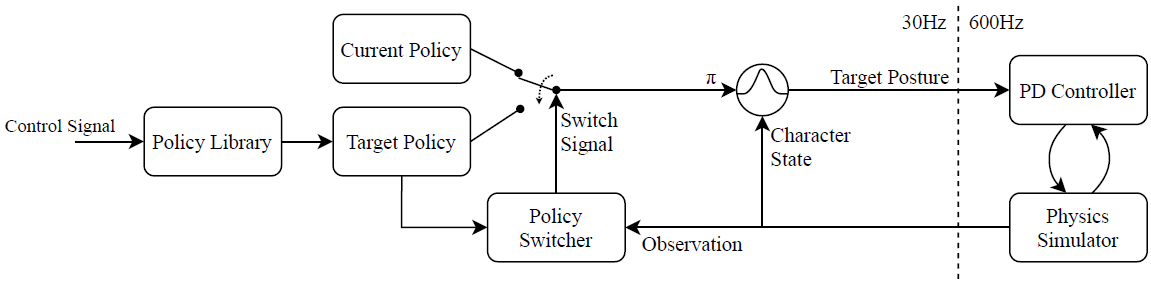
\includegraphics[width=0.85\textwidth]{Pictures/gail.png}
    \caption{GAIL: The policy switcher uses the character’s observation to decide whether to keep the currently activated policy or to switch to the target policy interactively responding to the external control signal when such a transition is considered feasible.}
    \label{fig:keypoints}
\end{figure}

The ICCGAN formulation~\cite{iccgan2021} stabilises training through three mechanisms: (i)~an ensemble of discriminators with shared feature layers but independent output heads, resisting overfitting; (ii)~hinge-loss optimization bounding scores to $[-1,\,1]$; and (iii)~gradient penalty regularisation~\cite{wgangp2017} enforcing Lipschitz smoothness. The discriminator ensemble score serves directly as the RL reward for PPO~\cite{ppo2017}, eliminating manual reward functions. The policy uses a GRU-based recurrent encoder operating on recent root-relative body-part observations, performing causal inference without phase counters or target poses---enabling interactive runtime switching between behaviours.

This GAN-like approach achieves state-of-the-art imitation performance without manually designing and fine-tuning a reward function. The policies directly control the character without having to track any target reference pose explicitly or implicitly through a phase state. The system can respond to external control signals provided by the user and interactively switch between different policies without requiring any motion generation or motion matching mechanism.

\subsection{Composite Motion and Task Control}

Single-clip imitation cannot produce composite behaviours such as locomotion with simultaneous upper-body manipulation. Despite significant advancements in physics-based character control, the majority of existing techniques rely on reference data consisting of motion capture recordings of an expert performing the behavior of interest. While such reference data is paramount to train motor control policies that lead to natural and robust control, we are interested in synthesizing composite behaviors for physically simulated humanoids by combining multiple motion capture reference clips into the training of a single policy. Further, we augment these imitation controllers with task-specific rewards to train the policy to accomplish specific functional tasks at the same time.

Assigning separate discriminators to body-part groups and aggregating their rewards via multi-objective weighting~\cite{composite2023} addresses this limitation. The core difference from existing imitation learning approaches is decoupling full-body control during training, turning imitation and goal-directed full-body training into a multi-objective learning framework. We extend GAN-style reinforcement learning and introduce a multi-objective learning framework to support multiple discriminators and automatic weighting of imitation and goal-driven subtask rewards. We propose an incremental learning scheme that uses a meta-policy from an existing behavior to augment the behavior with new subtasks, producing a composite motion control policy that can be learned significantly faster than learning from scratch. Our scheme automatically learns weights across the body that are state dependent in order to effectively mix the original behavior with a new subtask in a temporally dynamic fashion.

A multi-critic value function with per-component heads stabilises learning under competing gradients. Goal-conditioned extensions introduce spatial target-reaching and directional alignment rewards, while incremental training reuses pre-trained locomotion policies as meta-policies for efficient composite skill acquisition. The framework supports composite multi-objective control policies trained from decoupled motion sources without requiring pre-composed reference clips.

\subsection{Symmetry and Phase Priors}

Bilateral symmetry losses~\cite{symlocom2018} penalise differences between mirrored left-right joint actions, producing symmetric low-energy gaits without motion-capture data. Phase-functioned neural networks~\cite{phasefunc2017} condition locomotion controllers on the gait cycle phase, encoding contact timing as $(\sin 2\pi\phi,\, \cos 2\pi\phi)$. Both serve as auxiliary signals explored in our training pipeline, with empirical analysis presented in the experiments.

\subsection{Policy Adaptation}

A trained imitation policy may degrade under environmental change---new terrains, altered morphology, or modified task objectives. AdaptNet~\cite{adaptnet2023} proposes a two-tier adaptation hierarchy: the first tier augments latent state embeddings for modest behavioural shifts, the second modifies deeper network layers for substantial changes, achieving rapid adaptation while preserving stylistic qualities. This constitutes the planned third stage of our pipeline.
